\begin{exercice}

 Ci-dessous la courbe de la fonction $f$ d�finie sur $\R$ par:
\[f(x)=\e^{-x^2}\]
On cherche � trouver par diverses m�thodes une valeur approch�e de:
\[I=\int_{0}^{1}\e^{-x^2}\ud x\]
\begin{enumerate}
\item Justifier par un raisonnement graphique que: $2I=\int_{-1}^{1}\e^{-x^2}\ud x$
\item Justifier l'encadrement: $0 \leq I\leq 1$
\item D�terminer une valeur approch�e de $I$ � l'aide de la calculette.
\item En utilisant le quadrillage, d�terminer un encadrement de $I$. (Amplitude au plus 0,2)
\item En utilisant le point d'abscisse $0,3$ et deux trap�zes,
  d�terminer une nouvelle valeur approch�e de~$I$.
\item Comme on ne sait pas trouver de primitive de $f$, une technique
  consiste � trouver un polyn�me \og assez proche\fg{} de $f$ et d'en
  calculer l'int�grale sur le m�me intervalle. D�terminer le polyn�me $P$
  de degr� trois tel que:
\[ P(0)=f(0),\quad P'(0)=f'(0),\quad P(1)=f(1),\quad P'(1)=f'(1) \]
\item V�rifier � l'aide de la calculette que la courbe de $P$ est
  assez proche de celle de $f$ sur $\intf{0}{1}$. Est-ce le cas sur $\intf{-1}{1}$?
\item En d�duire une nouvelle valeur approch�e de $I$.
\item Prouver que le domaine compris entre la courbe et l'axe des
  abscisses, pour $x\geq 1$ est d'aire finie, en donner un encadrement. \emph{On pourra comparer
  $f(x)$ et $xf(x)$.}
\item Conclure en donnant une valeur approch�e de:
\[\int_{-\infty}^{+\infty}\e^{-x^2}\ud x\]
La valeur exacte est $\sqrt \pi$
\end{enumerate}
\noindent
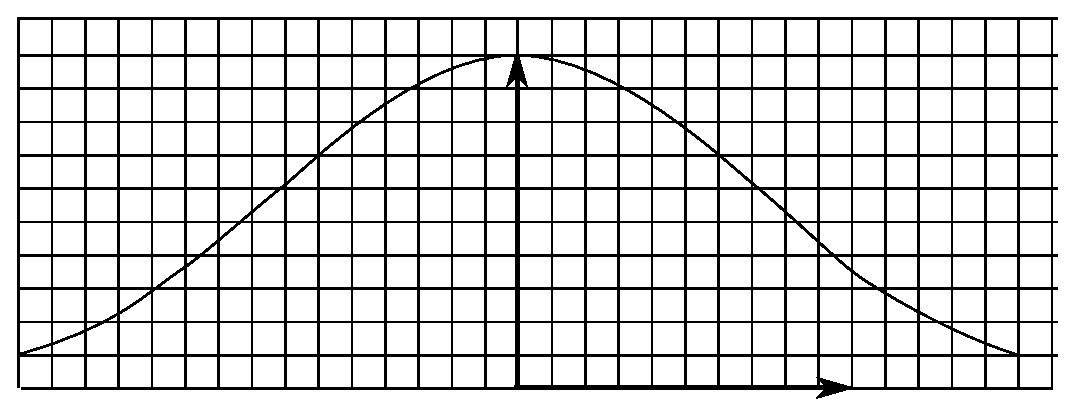
\includegraphics[width=15cm]{\CHEMIN/Integration/Exos/exo-7_13/Gaussienne}
\end{exercice}
